\documentclass[runningheads]{llncs}

\usepackage[UTF8]{ctex}
\usepackage{graphicx}
\usepackage{amsmath}
\usepackage{amssymb}
\usepackage{booktabs}
\usepackage{array}
\usepackage{url}

\newcommand{\figplaceholder}[2]{%
\fbox{%
\begin{minipage}[c][0.20\textheight][c]{0.92\textwidth}
\centering
\textbf{#1}\\[0.8em]
#2
\end{minipage}}}

\begin{document}

\title{面向非接触式压力识别的区域-时间注意力多区域颜色脉动网络}
\titlerunning{用于非接触式压力识别的 RT-MRCPNet}

\author{匿名作者}
\authorrunning{匿名作者}
\institute{匿名单位}

\maketitle

\begin{abstract}
压力往往先表现为生理变化，然后才可能表现为明显的面部表情或行为变化。因此，基于普通摄像头的人脸视频压力识别具有很强的应用吸引力，但也面临一个核心困难：有用的皮肤颜色变化十分微弱，在面部不同区域上的分布并不均匀，并且容易被运动、光照和身份外观淹没。现有视频方法大多沿着两条路线展开：一类直接对完整人脸帧建模，另一类先恢复远程生理信号，再计算特征进行分类。前者在小规模压力数据集上容易学习到身份或场景捷径，后者则可能过早压缩区域差异。为此，本文提出区域-时间注意力多区域颜色脉动网络 RT-MRCPNet。该方法将人脸视频片段转化为多个面部区域的 RGB 颜色时序序列，将不同区域视为多路弱生理观测。模型使用共享时序编码器提取区域内部颜色动态，通过时间注意力选择每个区域中更可靠的片段，并通过区域注意力自适应融合不同面部区域，最终得到片段级压力表示。本文在社会压力人脸视频数据上采用 subject-independent 协议进行实验，RT-MRCPNet 达到 88.42\% ACC、88.15\% F1-score 和 91.54\% AUC；相比最强轻量视频基线分别提升 1.89、2.27 和 2.33 个百分点，相比多区域固定融合基线分别提升 4.80、5.11 和 5.10 个百分点。

\keywords{非接触式压力识别 \and 人脸视频 \and 远程光电容积脉搏波 \and 颜色脉动序列 \and 区域-时间注意力}
\end{abstract}

\section{引言}

压力识别真正有价值的场景，往往不在实验室里。在线面试、远程学习、远程医疗和日常工作负荷监测都需要低打扰、易部署的感知方式。普通摄像头提供了一种自然的非接触式信号来源：人脸视频不仅记录表情、视线和头部运动，也包含由血容量变化引起的微弱皮肤颜色波动。已有远程光电容积脉搏波研究表明，这类颜色波动可以用于心率估计、心率变异性分析、情绪状态监测和压力相关推断~\cite{mcduff2014remote,benezeth2018remotehrv,nikolaiev2020noncontact}；UBFC-Phys、StressID 和 ForDigitStress 等数据集也进一步将人脸视频放入社会压力或数字交互协议中~\cite{sabour2021ubfcphys,chaptoukaev2023stressid,heimerl2024fordigitstress}。因此，基于人脸视频的非接触式压力识别具有明确应用价值，但其关键困难在于压力相关颜色变化微弱、局部且容易被身份外观、运动和光照变化淹没。

现有人脸视频方法容易在“完整视觉建模”和“全局生理信号摘要”之间损失有效证据。完整视频模型保留丰富外观细节，DeepPhys、PhysNet、MTTS-CAN 和 EfficientPhys 等工作证明深度网络可以学习远程生理表示~\cite{chen2018deepphys,yu2019physnet,liu2020mttscan,liu2023efficientphys}，但小规模压力数据使其容易学习身份、背景、肤色或任务场景等捷径。传统流程则先恢复全脸 rPPG 信号，再分类心率或心率变异性特征~\cite{mcduff2014remote,nikolaiev2020noncontact}，但这可能过早压缩额头、脸颊、鼻部和下巴之间的差异。由于不同面部区域的 rPPG 质量并不相同~\cite{zhao2020multiscale,xiong2023graphphys,bondarenko2025regions}，非接触式压力识别需要一种紧凑且保留区域证据的表示。

另一个挑战是压力视频中时间位置和面部区域的可靠性会动态变化。说话、计算、眨眼、转头、遮挡、反光和非对称光照可能在不同时间污染不同区域，固定平均会把有效反应与噪声片段混合。注意力机制可以根据输入为时间位置和区域分配权重，已有生理视频方法也使用注意力增强远程生理测量或压力识别~\cite{chen2018deepphys,liu2020mttscan,xu2024mtasr}。不过，对于样本有限的压力数据集，轻量注意力设计比大规模 Transformer 式模型更适合。

本文提出 RT-MRCPNet，即区域-时间注意力多区域颜色脉动网络。该方法将面部区域视为多路弱生理观测源，直接从区域 RGB 动态中学习压力相关表示；时间注意力用于选择每个区域内更可靠的片段，区域注意力用于融合更有判别力的面部区域。本文贡献包括：（1）将视频压力识别建模为多区域颜色脉动序列学习问题；（2）设计轻量区域-时间注意力网络，分别建模时间可靠性和区域贡献；（3）在 UBFC-Phys 跨被试协议下验证方法，RT-MRCPNet 达到 88.42\% ACC、88.15\% F1-score 和 91.54\% AUC，优于全脸 RGB、单区域、多区域固定融合、传统 rPPG 特征和轻量视频基线。

\section{相关工作}

\subsection{压力识别与多模态数据}

压力识别长期依赖心电、皮肤电、光电容积脉搏波、呼吸和皮肤温度等接触式生理信号，因为它们接近压力反应机制~\cite{healey2005drivingstress,schmidt2018wesad,schmidt2019wearableaffectreview}。心率变异性描述自主神经调节，皮肤电反映交感唤醒，呼吸节律也会随认知负荷变化，但这些传感器需要佩戴、同步和用户配合~\cite{schmidt2018wesad,bota2022empathicschool}。因此，近年数据集开始走向更真实的多模态场景：UBFC-Phys 在静息、演讲和算术任务中采集人脸视频以及腕带 BVP 和 EDA~\cite{sabour2021ubfcphys}；StressID 在情绪、认知和公开演讲刺激下记录视频、音频、ECG、EDA 和呼吸~\cite{chaptoukaev2023stressid}；ForDigitStress 面向数字化面试，包含视频、眼动、音频、PPG 和 EDA~\cite{heimerl2024fordigitstress}。这些数据集推动了非接触式压力识别，也说明高质量压力数据仍然规模有限且依赖具体协议。

\subsection{非接触式压力识别与人脸颜色线索}

早期非接触式研究通常先从人脸视频估计远程生理指标，再用于分类。McDuff 等~\cite{mcduff2014remote} 利用视频估计心率、呼吸和心率变异性并进行认知压力分类；Nikolaiev 等~\cite{nikolaiev2020noncontact} 从普通摄像头 rPPG 中恢复 HRV 指标；Benezeth 等~\cite{benezeth2018remotehrv} 探索远程 HRV 在情绪监测中的作用。近期工作开始转向直接视频学习：Xu 等~\cite{xu2024mtasr} 使用多任务学习和峰值注意力进行人脸视频压力识别，SympCam~\cite{braun2024sympcam} 及相关研究~\cite{braun2023sympathetic} 则从面部和手部视频估计交感唤醒。这些研究表明，压力识别与 rPPG 相关，但并不等同于恢复一条干净脉搏波；判别线索可能表现为局部颜色动态、短时峰值或任务诱发的说话和运动。

传统 rPPG 方法如 CHROM~\cite{dehaan2013chrom}、POS~\cite{wang2017pos} 和 LGI~\cite{pilz2018lgi} 说明 RGB 轨迹包含弱心血管信息；DeepPhys~\cite{chen2018deepphys}、PhysNet~\cite{yu2019physnet}、MTTS-CAN~\cite{liu2020mttscan} 和 EfficientPhys~\cite{liu2023efficientphys} 进一步从视频时空变化中学习生理证据。不过，这些方法通常以生命体征估计为目标，评价重点是波形质量或心率误差。压力识别更关注心理或社会任务诱发的判别模式，因此需要将远程生理颜色线索转化为适合分类的表示。

\subsection{多区域建模与注意力机制}

面部区域选择是 rPPG 质量的关键因素，因为局部血流、皮肤纹理、姿态、光照和运动会导致不同 ROI 的信噪比差异。多尺度和多 ROI 方法可以提升心率估计鲁棒性~\cite{zhao2020multiscale}，近期研究也指出区域选择仍是开放问题~\cite{bondarenko2025regions}，GraphPhys 则用图神经网络建模面部区域关系~\cite{xiong2023graphphys}。注意力机制同样常用于抑制背景或不可靠帧，并突出有效波形片段。然而，现有注意力设计多服务于完整视频表征或远程生理重建。本文关注的是更聚焦的问题：能否使用紧凑区域颜色序列，并通过两个轻量注意力阶段分别完成区域内部时间聚合和区域之间贡献融合，从而提升 subject-independent 压力识别。

\section{方法}

\subsection{问题定义}

给定人脸视频片段 $V=\{I_1,I_2,\ldots,I_T\}$，目标是预测二分类标签 $y \in \{0,1\}$，其中 $0$ 表示非压力，$1$ 表示压力。视频被表示为
\begin{equation}
    X \in \mathbb{R}^{K \times T \times C},
\end{equation}
其中 $K$ 表示面部区域数量，$T$ 表示片段长度，$C=3$ 表示 RGB 三个颜色通道。对于一个 batch，模型输入为 $X \in \mathbb{R}^{B \times K \times T \times C}$。

\subsection{多区域颜色脉动表示}

对于每一帧，首先检测、裁剪并缩放人脸，使固定 ROI 在不同帧间保持几何一致。图~\ref{fig:region_partition_zh} 展示了本文使用的五个区域：额头、左脸颊、右脸颊、鼻部和下巴。它们覆盖 rPPG 常用皮肤区域，同时具有不同可靠性：脸颊通常包含较清晰的颜色动态，额头较稳定但可能受头发影响，鼻部易受高光影响，下巴易受说话动作干扰。

\begin{figure}
\centering
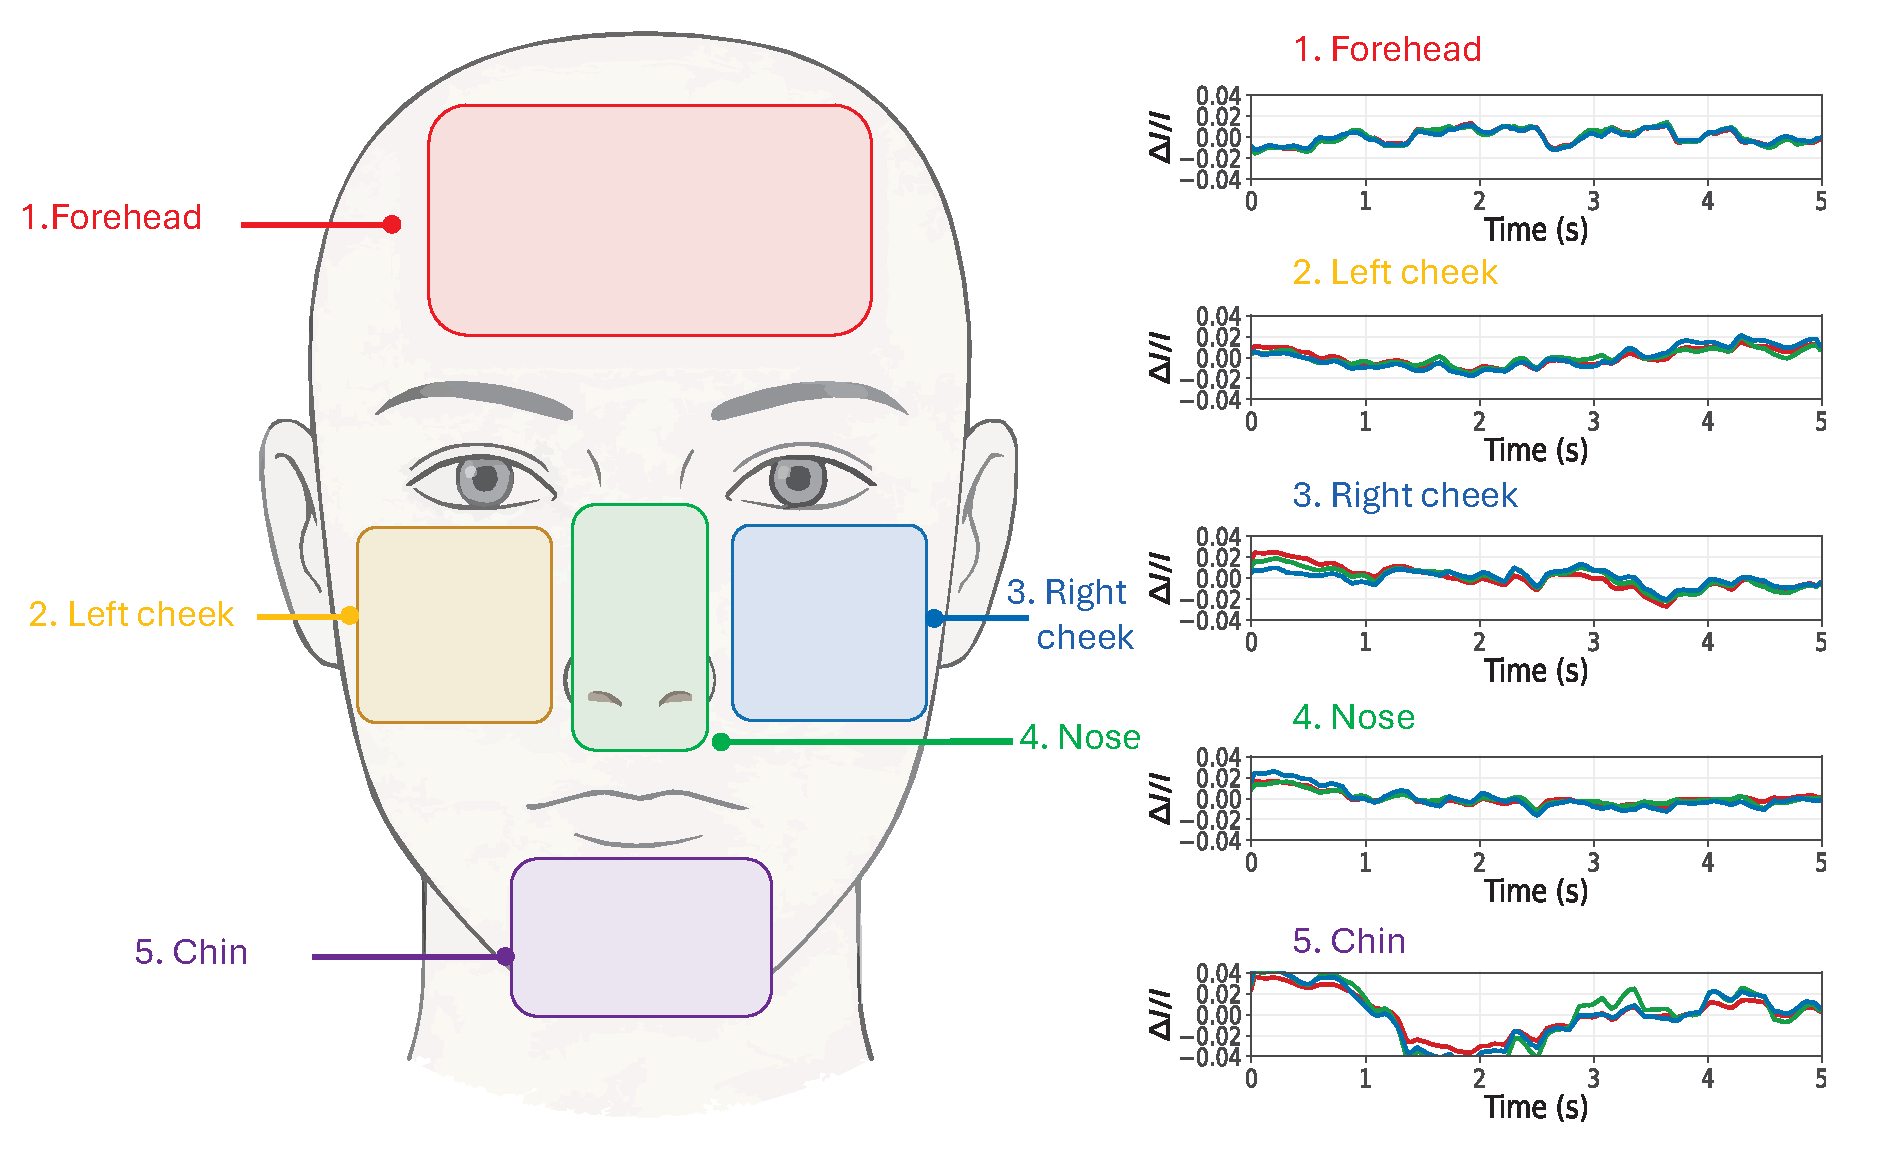
\includegraphics[width=0.98\textwidth]{f2.eps}
\caption{本文多区域颜色脉动表示使用的五个面部区域。}
\label{fig:region_partition_zh}
\end{figure}

对于第 $k$ 个区域在第 $t$ 帧上的 RGB 向量，本文使用区域内所有像素的平均值：
\begin{equation}
    x_{k,t} = \frac{1}{|\Omega_k|} \sum_{p \in \Omega_k} I_t(p),
\end{equation}
其中 $\Omega_k$ 表示第 $k$ 个区域的像素集合。第 $k$ 个区域的颜色序列可以表示为
\begin{equation}
    X_k = [x_{k,1}, x_{k,2}, \ldots, x_{k,T}].
\end{equation}
将所有区域序列堆叠后得到 $X \in \mathbb{R}^{K \times T \times C}$，其中 $C=3$，对应 RGB 三个颜色通道。

本文对每个区域、每个颜色通道分别进行时间维度标准化：
\begin{equation}
    \hat{X}_{k,:,c} = \frac{X_{k,:,c} - \mu_{k,c}}{\sigma_{k,c}+\epsilon}.
\end{equation}
其中，$\hat{X}$ 表示标准化序列，$c$ 为颜色通道索引，$\mu_{k,c}$ 和 $\sigma_{k,c}$ 为片段内均值和标准差，$\epsilon$ 防止除零。该表示去除大部分空间冗余，同时保留区域颜色动态。

\subsection{区域时序编码器}

每个区域序列由共享的一维时序编码器进行编码。给定标准化张量 $\hat{X}$，先将其调整为 $\tilde{X}$，再输入多层一维卷积块：
\begin{equation}
    H = E_{\theta}(\tilde{X}),
\end{equation}
经过维度调整后，$H \in \mathbb{R}^{B K \times T \times D}$，其中 $D$ 为隐藏维度。记 $h_{k,t} \in \mathbb{R}^{D}$ 为第 $k$ 个区域在第 $t$ 个时间位置的特征。共享编码器可以捕获不同区域共有的低层颜色动态，同时降低参数量和过拟合风险；短时间卷积核则用于建模局部变化，而无需反复处理完整空间图像网格。

\subsection{时间注意力}

对于第 $k$ 个区域的时序特征，时间注意力为每个时间位置预测一个分数：
\begin{equation}
    e_{k,t} = \mathbf{w}_t^\top \tanh(\mathbf{W}_t h_{k,t}),
\end{equation}
其中 $\mathbf{W}_t$ 为时间注意力中的特征投影矩阵，$\mathbf{w}_t$ 为用于生成标量分数的权重向量。归一化后的时间权重为
\begin{equation}
    \alpha_{k,t} = \frac{\exp(e_{k,t})}{\sum_{\tau=1}^{T}\exp(e_{k,\tau})}.
\end{equation}
区域级表示通过加权求和得到：
\begin{equation}
    r_k = \sum_{t=1}^{T}\alpha_{k,t} h_{k,t}.
\end{equation}
这样，每个区域拥有独立时间权重，可以在区域融合前抑制说话、运动或光照造成的不稳定片段。

\subsection{区域注意力}

完成时间聚合后，模型得到区域级表示 $\{r_1,\ldots,r_K\}$。区域注意力首先为每个区域计算贡献分数：
\begin{equation}
    s_k = \mathbf{w}_r^\top \tanh(\mathbf{W}_r r_k),
\end{equation}
其中 $\mathbf{W}_r$ 为区域注意力中的特征投影矩阵，$\mathbf{w}_r$ 为用于生成区域标量分数的权重向量。然后通过 softmax 得到区域权重：
\begin{equation}
    \beta_k = \frac{\exp(s_k)}{\sum_{j=1}^{K}\exp(s_j)}.
\end{equation}
注意力融合后的片段级表示为
\begin{equation}
    z_{\mathrm{attn}} = \sum_{k=1}^{K}\beta_k r_k.
\end{equation}
为了提升训练稳定性，本文加入平均区域表示作为残差项：
\begin{equation}
    z = z_{\mathrm{attn}} + \frac{1}{K}\sum_{k=1}^{K} r_k.
\end{equation}
最终，$z$ 输入两层 MLP 分类器，得到 logits：
\begin{equation}
    o = \mathrm{MLP}(z).
\end{equation}

图~\ref{fig:overview_zh} 总结了 RT-MRCPNet 的整体流程。

\begin{figure}
\centering

\includegraphics[width=0.98\textwidth]{f1.eps}
\caption{RT-MRCPNet 模型结构图。}
\label{fig:overview_zh}
\end{figure}

\subsection{训练目标}

本文使用交叉熵损失训练模型。令 $p_c=\mathrm{softmax}(o)_c$ 表示类别 $c$ 的预测概率，则损失函数为
\begin{equation}
    \mathcal{L}_{cls} = -\sum_{c=1}^{2} y_c \log p_c,
\end{equation}
其中 $y_c$ 表示真实标签的 one-hot 编码在类别 $c$ 上的取值。本文只使用分类监督，使比较聚焦于区域 RGB 动态和注意力聚合。

\section{实验}

\subsection{数据集与标签定义}

本文主要实验使用 UBFC-Phys 类型社会压力人脸视频。T1 为静息任务，标记为非压力（$y=0$）；T2 和 T3 分别为演讲和算术任务，标记为压力（$y=1$）。

\subsection{Subject-Independent 协议}

所有实验均采用 subject-independent 划分，即同一被试的视频片段不能同时出现在训练集和测试集中。固定划分使用 70\% 被试训练、15\% 被试验证、15\% 被试测试，并根据验证集 F1-score 选择 checkpoint。

\subsection{实现细节}

人脸被裁剪到 $128 \times 128$，并划分为长度 $T=160$ 的片段。本文使用五个固定 ROI，提取逐帧 RGB 均值序列并进行时间标准化。模型隐藏维度为 128，使用 AdamW 优化器，初始学习率为 $10^{-3}$，batch size 为 64，训练 100 轮，并在单张 NVIDIA RTX 3090 上用 PyTorch 2.1 实现。

\subsection{评价指标}

本文报告 Accuracy、F1-score 和 AUC，并将压力状态视为正类。

\subsection{对比实验}

在输入形式允许的情况下，所有方法使用同一输入来源、跨被试划分、片段构造方式和评价代码。全脸 RGB、单区域 RGB 和多区域固定融合为本文构造的基线；传统 rPPG、视频时序模型和 rPPG backbone 参考已有方法或网络结构实现。
\begin{itemize}
    \item 全脸 RGB 时序网络：将五个区域序列先平均为一个全脸级 RGB 序列，再进行时序编码。
    \item 单区域 RGB 时序网络：分别使用额头、左脸颊、右脸颊、鼻部和下巴区域，用于观察不同面部区域的识别差异。
    \item 多区域固定融合：保留多个区域 RGB 序列，但使用非自适应拼接或平均融合，不使用注意力。
    \item 传统 rPPG 特征分类器：从面部颜色轨迹中提取 POS 或 CHROM 风格信号~\cite{wang2017pos,dehaan2013chrom}。随后计算 HR/HRV 等手工特征，并使用 SVM 或随机森林分类。
    \item 轻量视频时序基线：使用紧凑 CNN-LSTM 或 3D CNN 直接输入裁剪后的人脸片段，输出压力类别。CNN-LSTM 类结构参考远程压力估计中的 CCT-LSTM 思路~\cite{ziaratnia2024cctlstm}，3D CNN 类结构参考经典三维卷积视频建模方法~\cite{tran2015c3d}。
    \item 已有 rPPG backbone 加压力分类头：将 PhysNet~\cite{yu2019physnet} 或 EfficientPhys~\cite{liu2023efficientphys} 等代表性 rPPG 模型的输出头替换为压力分类头。
    \item RT-MRCPNet：本文方法，使用多区域 RGB 序列，并通过时间注意力和区域注意力进行自适应融合。
\end{itemize}

\begin{table}
\caption{UBFC-Phys subject-independent 统一协议下的对比实验。所有指标均以百分比（\%）报告。}
\label{tab:main_results_zh}
\centering
\small
\begin{tabular}{p{3.6cm}p{4.1cm}ccc}
\toprule
方法 & 输入 & ACC & F1 & AUC \\
\midrule
全脸 RGB 时序网络 & 全脸平均 RGB 序列 & 81.42 & 80.85 & 84.51 \\
额头单区域时序网络 & 额头 RGB 序列 & 79.80 & 78.64 & 82.05 \\
左脸颊单区域时序网络 & 左脸颊 RGB 序列 & 82.55 & 81.72 & 85.23 \\
右脸颊单区域时序网络 & 右脸颊 RGB 序列 & 82.14 & 81.48 & 84.81 \\
鼻部单区域时序网络 & 鼻部 RGB 序列 & 76.40 & 75.12 & 79.55 \\
下巴单区域时序网络 & 下巴 RGB 序列 & 77.85 & 76.50 & 80.12 \\
多区域固定融合 & 五个 ROI RGB 序列，固定融合 & 83.62 & 83.04 & 86.44 \\
rPPG 特征 + SVM & HR/HRV 手工特征 & 78.50 & 77.25 & 81.33 \\
rPPG 特征 + 随机森林 & HR/HRV 手工特征 & 80.25 & 79.52 & 83.10 \\
轻量 CNN-LSTM & 裁剪人脸片段 & 84.20 & 83.55 & 87.12 \\
轻量 3D CNN & 裁剪人脸片段 & 85.15 & 84.78 & 88.02 \\
PhysNet/EfficientPhys + 压力分类头 & 人脸片段或 rPPG 相关特征 & 86.53 & 85.88 & 89.21 \\
RT-MRCPNet & 五个 ROI RGB 序列，注意力融合 & \textbf{88.42} & \textbf{88.15} & \textbf{91.54} \\
\bottomrule
\end{tabular}
\end{table}

\begin{figure}
\centering
\IfFileExists{fig3_attention_reliability.eps}{%
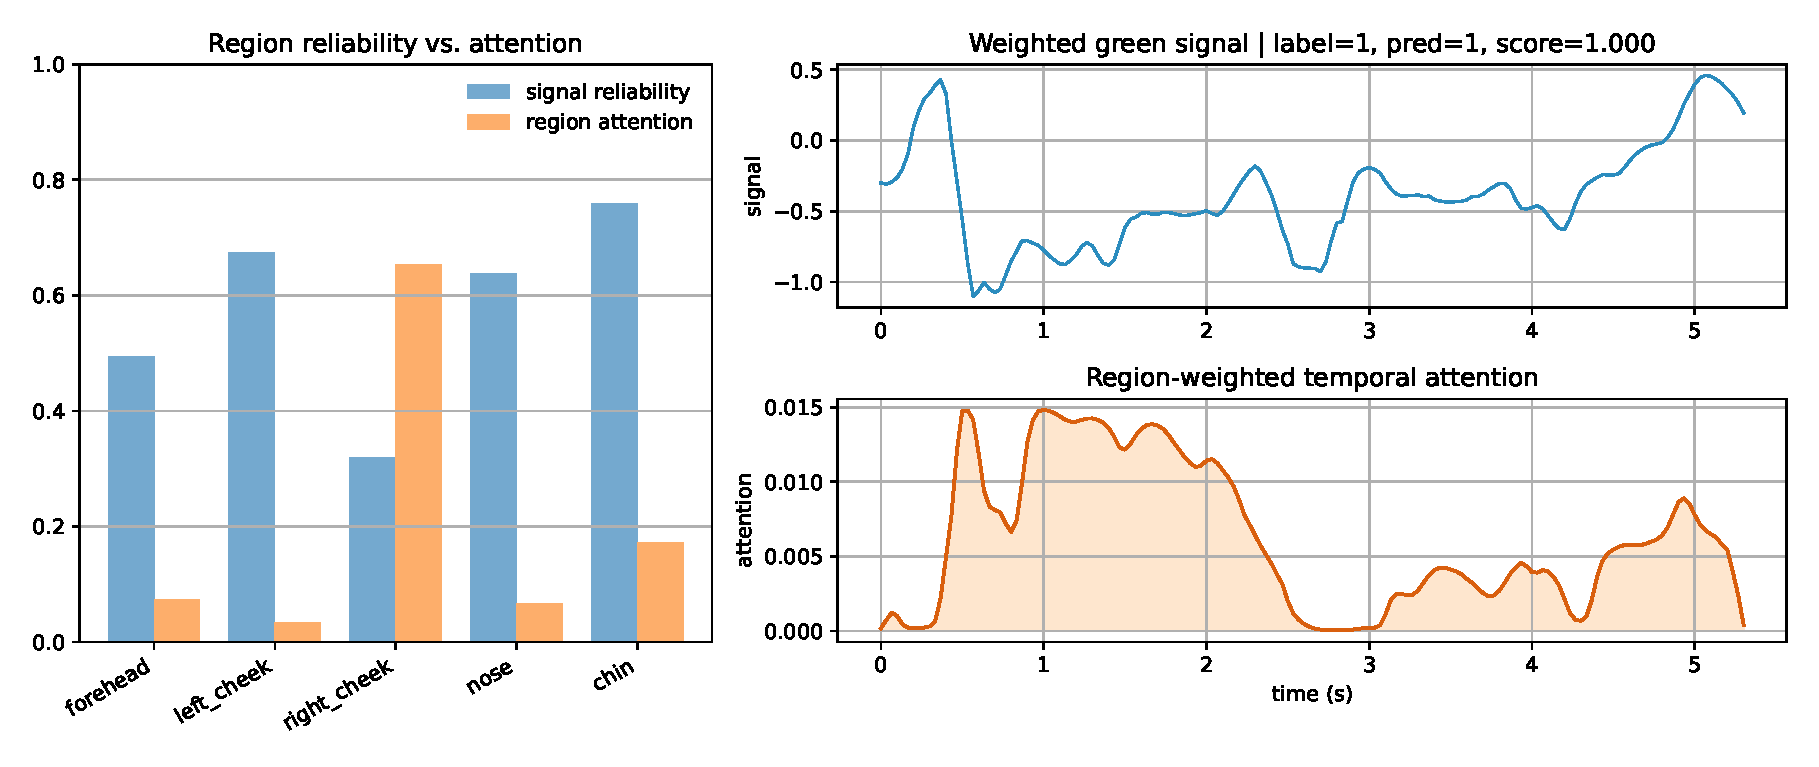
\includegraphics[width=0.92\textwidth,height=0.18\textheight,keepaspectratio]{fig3_attention_reliability.eps}%
}{%
\figplaceholder{图 3 注意力可靠性可视化}{展示代表性片段中的注意力权重分布，用于分析模型如何降低不稳定时间位置和低质量区域的影响。}%
}
\caption{注意力可靠性可视化。}
\label{fig:attention_reliability_zh}
\end{figure}

表~\ref{tab:main_results_zh} 和图~\ref{fig:attention_reliability_zh} 表明，RT-MRCPNet 在 RGB 序列、传统 rPPG 特征和轻量视频基线中取得最佳结果。单区域结果中，左右脸颊优于鼻部和下巴，说明区域信号质量并不均匀。全脸平均会混合稳定区域和受说话、反光或遮挡影响的区域，多区域固定融合也默认所有区域同等可靠。RT-MRCPNet 保留多区域独立观测，并通过时间注意力和区域注意力自适应选择可靠片段和面部区域，避免过早压缩为单一全局 rPPG 信号，也避免训练较重的完整视频模型，因此更适合 subject-independent 小规模压力识别。

\subsection{消融实验}

消融实验采用与表~\ref{tab:main_results_zh} 相同的协议，并从 RT-MRCPNet 中移除具体注意力模块。

\begin{table}
\caption{RT-MRCPNet 消融实验。所有指标均以百分比（\%）报告。}
\label{tab:ablation_zh}
\centering
\begin{tabular}{lccc}
\toprule
模型变体 & ACC & F1 & AUC \\
\midrule
无注意力 & 83.62 & 83.04 & 86.44 \\
仅时间注意力 & 86.15 & 85.52 & 88.90 \\
仅区域注意力 & 85.34 & 84.71 & 88.22 \\
完整 RT-MRCPNet & \textbf{88.42} & \textbf{88.15} & \textbf{91.54} \\
\bottomrule
\end{tabular}
\end{table}

消融结果表明两个注意力阶段具有互补作用。无注意力模型退化为固定融合，难以处理短时扰动和区域质量差异；时间注意力可以弱化每个 ROI 内的不稳定时刻，区域注意力可以提高可靠面部区域的贡献。完整 RT-MRCPNet 取得最佳结果，说明压力相关证据同时具有时间选择性和区域差异。图~\ref{fig:region_signal_diversity_zh} 进一步展示了区域颜色序列差异。

\begin{figure}
\centering
\IfFileExists{fig4_region_signal_diversity.eps}{%
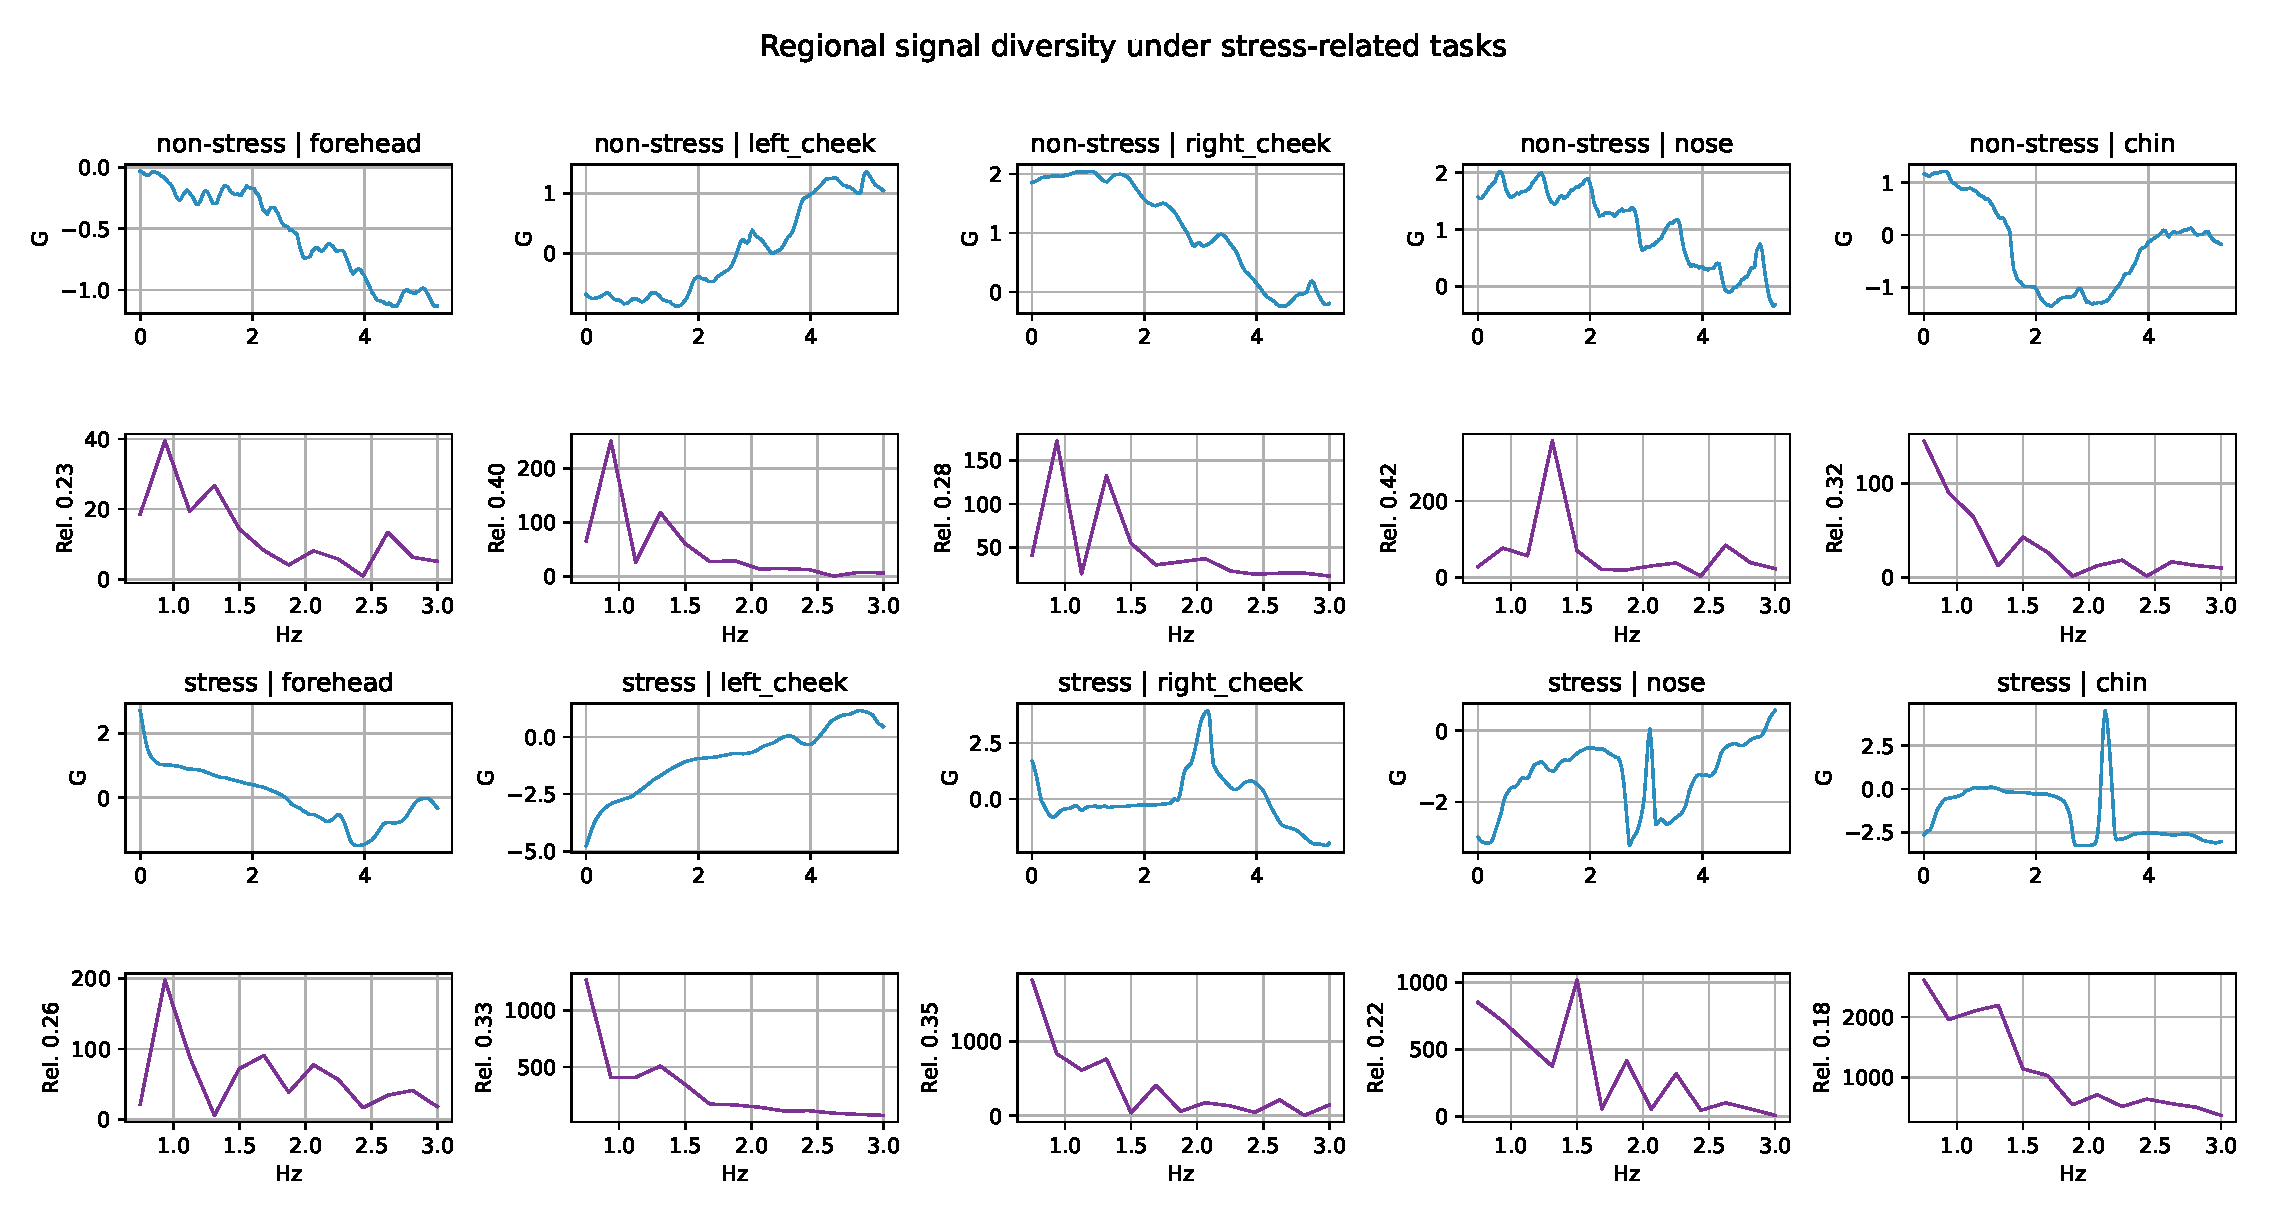
\includegraphics[width=0.92\textwidth,height=0.18\textheight,keepaspectratio]{fig4_region_signal_diversity.eps}%
}{%
\figplaceholder{图 4 区域信号差异可视化}{展示不同面部 ROI 的颜色序列差异，用于说明各区域信号质量和判别贡献并不相同。}%
}
\caption{区域信号差异可视化。}
\label{fig:region_signal_diversity_zh}
\end{figure}

\subsection{复杂度分析}

对于长度为 $T$、分辨率为 $H \times W$ 的人脸视频，完整帧模型的输入规模为
\begin{equation}
    \mathcal{O}(T H W C),
\end{equation}
预处理后，RT-MRCPNet 只保留 $K$ 个区域的颜色均值序列：
\begin{equation}
    \mathcal{O}(K T C).
\end{equation}
由于 $K \ll H W$，该表示在进入神经网络前显著降低了空间冗余。

设隐藏维度为 $D$，卷积核大小为 $q$，编码层数为 $L$，时序编码主要复杂度为
\begin{equation}
    \mathcal{O}(B K L T q D^2),
\end{equation}
其中 $B$ 为 batch size。时间注意力和区域注意力的额外开销为
\begin{equation}
    \mathcal{O}(B K T D + B K D),
\end{equation}
相对于完整帧视频建模较小。RT-MRCPNet 的计算量主要随 $K$ 和 $T$ 增长，而不是随图像面积 $H W$ 增长。表~\ref{tab:complexity_zh} 报告了实际复杂度。

\begin{table}
\caption{模型复杂度对比。FLOPs 表示浮点运算量。}
\label{tab:complexity_zh}
\centering
\begin{tabular}{lccc}
\toprule
方法 & 参数量 & FLOPs & 推理时间 \\
\midrule
完整帧卷积循环网络 & 12.54M & 15.20G & 35.42 ms \\
完整帧三维卷积网络 & 33.25M & 38.64G & 42.15 ms \\
全脸 RGB 时序网络 & 0.82M & 0.05G & 1.25 ms \\
RT-MRCPNet & 0.94M & 0.25G & 2.38 ms \\
\bottomrule
\end{tabular}
\end{table}

\section{结论}

本文提出 RT-MRCPNet，一种用于非接触式压力识别的轻量级区域-时间注意力网络。该方法将人脸视频转化为多区域 RGB 时序序列，使用共享编码器建模局部颜色动态，并通过时间注意力和区域注意力聚合信息。在 subject-independent 协议下，RT-MRCPNet 达到 88.42\% ACC、88.15\% F1-score 和 91.54\% AUC。消融实验和复杂度分析表明，两个注意力阶段能够带来互补增益并保持较低计算开销。未来工作将探索自适应 ROI 定义、更细粒度压力标签和多模态融合。

\begingroup
\let\small\tiny
\bibliographystyle{splncs04_unsrt}
\bibliography{references}
\endgroup

\end{document}
